\section{Spark and the MapReduce Programming Model}

MapReduce is a programming model and an associated implementation that emerged to simplify common tasks associated with big data processing. These include managing parallel and distributed computing and ensuring fault tolerance of the computations \cite{Dean:2008:MSD:1327452.1327492}. The model is heavily influenced by functional programming, a programming paradigm that emphasises the use of pure functions and avoiding mutable state. As the name \textit{MapReduce} suggests, the computational model of a MapReduce system is based on two higher order functions, \textit{map} and \textit{reduce}. 

Spark is a MapReduce system implemented in the Scala programming language that is built around an abstraction called Distributed Resilient Datasets (RDDs)~\cite{Zaharia:2012:RDD:2228298.2228301}. The RDD abstration allows Spark to implement efficient fault tolerance. A common way of achieving fault tolerance is by maintaining multiple redundant copies of all datasets. Each time a dataset is mutated, all copies are mutated as well. While this certainly makes the system tolerant to lost datasets, it imposes quite significant overhead as each update needs to be replicated and extra space is required by the copies. Instead of maintaining redundant copies of each dataset, Spark solves the problem of fault tolerance by maintains the lineage of its datasets. The lineage of an RDD is a collection of instructions that specify how the RDD was computed from other RDDs. In case the Spark system loses an RDD, it can recreate the lost dataset by tracing its lineage back to existing RDDs and applying the instructions to recompute the lost dataset.       

The Spark runtime consists of a \textit{driver} application and one or more \textit{worker} application to which the driver application connects to and assigns tasks~\cite{Zaharia:2012:RDD:2228298.2228301}. In a typical scenario, the \textit{worker} applications reside on separate compute nodes of a computer cluster.

The programming interface that Spark provides is analogous to the collection library in the Scala standard library. The interface offers two types of functions: transformations that construct new RDDs from existing ones, such as \textit{map} and \textit{filter}, and actions that either save data to disk or return values to the application, such as \textit{collect} and \textit{reduce}~\cite{Zaharia:2012:RDD:2228298.2228301}. Transformations are computed lazily, which allows pipelining consecutive transformations and constructing a lineage graph of the computation before computation even takes place. Actions are used to execute work flows constructed by transformations and return the results to the application or write them to the disk. The map function, defined for class \textit{RDD[T]}, where \textit{T} is the element type parameter of the RDD, has essentially the following type signature

\[map[U](f: (T) \Rightarrow U): RDD[U]\]

The function produces a new RDD with element type \textit{U} by applying function \textit{f} to each element of the original RDD. Similarly, function \textit{filter} has the type signature

\[filter(f: (T) \Rightarrow Boolean): RDD[T]\]

and works by constructing a new RDD by including those elements of the original RDD where predicate \textit{f} is true. The action \textit{collect} has the simple type signature 

\[collect(): Array[T]\]

as it merely returns the results of the computation performed by transformations on the RDD to the application. The \textit{reduce} action has the signature

\[reduce(f: (T, T) \Rightarrow T): T\]

and it works conceptually by applying the binary operator \textit{f} iteratively to elements of the RDD until there is only one element left. The order and pairing of the elements is not specified to allow parallel computation and thus the operator needs to be commutative and associative in order to guarantee deterministic results. 

Let us look at a simple example to illustrate the usage of Spark. Suppose we have a text file where each line contains a decimal number and we wish to calculate the sum of all positive numbers in the file. The following Scala program implements this idea.  

\begin{minipage}{0.95\linewidth}
\begin{lstlisting}[language=scala] 
object SumNumbers {

  def initSpark(): SparkSession = {
    val sparkMaster = Properties
      .envOrNone("SPARK_MASTER").get

    SparkSession.builder()
      .appName("SumNumbers")
      .master(sparkMaster)
      .getOrCreate()
  }

  def main(args: Array[String]) {
    val session = initSpark()
    val sc = session.sparkContext

    val numbers: RDD[Double] = sc
      .textFile(args(0))
      .map(_.toDouble)
    val positive: RDD[Double] = numbers
      .filter( _ >= 0)
    val sum: Double = positive.reduce(_ + _)
    println(s"Sum of positive numbers is ${sum}")
  }
}        
\end{lstlisting}
\end{minipage}

Explicit type annotations are included at lines 17, 20 and 22 to clarify the execution context of values \textit{numbers}, \textit{positive} and \textit{sum}. The value \textit{numbers} as well as value \textit{positive} describe transformations applied to an RDD of strings, created at lines 17 and 18 by calling $sc.textFile(args(0))$. This reads the text file given as the first command line parameter to the program and creates an RDD whose elements are the lines in the text file. In line 19, the RDD of strings is converted to an RDD of double precision floating point values by applying method $toDouble$ to each element. In lines 20 to 21, the RDD of doubles is further transformed by calling \textit{filter(\_ >= 0)}. The filter function, as explained above, applies a predicate to the RDD returning a new RDD containing only the elements whose value is greater than or equal to zero. Finally, at line 22, the call to action \textit{positive.reduce} causes the computation defined by the RDD objects to materialize and calculates the sum of elements of RDD \textit{positive}. Readers who are not familiar with Scala programming language might find expressions such as $\_.toDouble$ and $\_ + \_$ slightly confusing. These expressions are merely syntactic sugar for expressing anonymous functions and can be written equivalently as $x => x.toDouble$ and $(x, y) => x + y$ respectively.

Each RDD consists of partitions, which are independent subdivisions of the dataset~\cite{Zaharia:2012:RDD:2228298.2228301}. Each partition may be computed in parallel or even on different machines. The programmer can control the number partitions that an RDD should be divided into by calling the RDD object's \textit{repartition} method and providing the desired number of partitions. Partitions have their individual lineage graph specifying which partitions of the parent RDDs they depend on. When executing a work flow, Spark groups together transformations that can be pipelined to form stages. An RDD operation that depends on multiple RDDs will create a stage boundary, because both dependency RDDs will need to be materialized before the operation can be executed.

Figure~\ref{figure:spark-example-dag} shows a lineage graph of the example work flow discussed above, assuming the default number of partitions is three. The tall rectangles represent RDDs and the small squares inside represent the partitions of the RDDs. Above each RDD is the name of the function that is responsible for creating the RDD. All the RDDs are wrapped inside a single stage, because the operations can be pipelined. The black arrows in between the partitions represent the lineage of the partitions.   

\begin{figure}[!htbp]
	\centering
	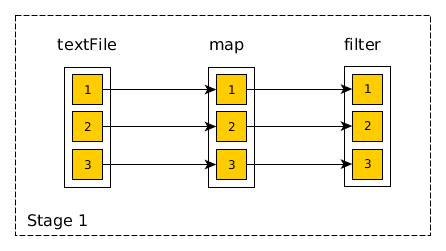
\includegraphics[scale=0.75]{images/spark_dag.png}
	\caption{Lineage graph of the example Spark work flow. Tall rectangles represent RDDs and squares inside them represent partitions.}
	\label{figure:spark-example-dag}
\end{figure}    